We present a new automated method for relative termination of double-pushout (DPO) graph rewriting systems with injective rules~\cite{corradini1997algebraic,habel2001double}.~\footnote{This work resulted in a publication at the 18th International Conference on Graph Transformation (ICGT 2025)~\cite{qiu2025termination_icgt}. Reproduced with permission from Springer Nature.} To prove the relative termination of a set of rules \(\mathcal{A}\) with respect to another set of rules \(\mathcal{B}\), the method requires identifying patterns whose counts decrease with each application of a rule from \(\mathcal{A}\) and do not increase with each application of a rule from \(\mathcal{B}\). 
Left-hand sides of the rules are typical examples of such patterns, and we leave it to future work to explore whether other patterns are useful.
 
Let \( \mathbb{X} \) denote a fixed set of patterns. We assign weights (natural numbers) to monomorphisms from graphs in \( \mathbb{X} \), and define the weight of a graph $G$ as the sum of the weights of all monomorphisms from graphs in \( \mathbb{X} \) to $G$. 
  
Let $\mathcal{A}$ and $\mathcal{B}$ be sets of DPO rewriting rules. Let $X \mathop{\in} \mathbb{X}$ and $G \mathop{\Rightarrow} H$ be a rewriting step defined by the double-pushouts diagram shown below. 
\begin{center}
     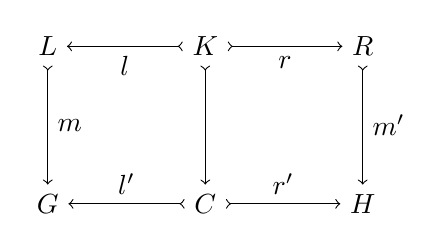
\begin{tikzpicture}
            \node (I) at (0,0) {$K$};
            \node (L)  at (-2,0) {$L$};
            \node (R)  at (2,0) {$R$};
            \node (G)  at (-2,-2) {$G$};
            \node (C)  at (0,-2) {$C$};
            \node (H)  at (2,-2) {$H$};
            \draw [>->] (I) to  node [midway,below] {$l$} (L);
            \draw [>->] (I) to  node [midway,below] {$r$} (R);
            \draw [>->] (L) to node [midway,right] {$m$} (G);
            \draw [>->] (I) to  node [midway,right] 
            {} (C);
            \draw [>->] (R) to  node [midway,right] 
            {$m'$}
            (H);
            \draw [>->] (C) to node [midway,above] {$l'$} (G);
            \draw [>->] (C) to node [midway,above] 
            {$r'$} 
            (H);
        \end{tikzpicture}
    \end{center}
The image of a monomorphism from $X$ to $G$ falls into exactly one of the following three mutually exclusive cases:
\begin{enumerate}
    \item the image is fully included in $m(L)$;
    \item the image is fully included in $l'(C)$; 
    \item the image is neither fully included in $m(L)$ nor fully included in $l'(C)$.
\end{enumerate} 
 Similary, the image of a monomorphism from $X$ to $H$ falls into exactly one of the following three mutually exclusive cases:
 \begin{enumerate}
    \item the image is fully included in $m'(R)$;
    \item the image is fully included in $r'(C)$;
    \item the image is neither fully included in $m'(R)$ nor fully included in $r'(C)$.
 \end{enumerate}
  The number of monomorphisms $h: X \to G$ whose image is fully included in $m(L)$ can be computed exactly; likewise, the number of monomorphisms $x: X \to H$ whose image is fully included in $m'(R)$ can be computed exactly. Moreover, the number of monomorphisms $x: X \to G$ whose image is fully included in $l'(C)$ equals to the number of monomorphisms $x: X \to H$ whose image is fully included in $r'(C)$. Therefore, to estimate the change in weight when applying a rewriting rule, it suffices to compare the numbers of monomorphisms in the third cases above.
  
  To enable this comparison, we suppose that for every $X \in \mathbb{X}$, 
  the following conditions hold: 
\begin{itemize}
    % \item For every rule in \( \mathcal{A} \), the left-hand side graph's weight is strictly greater than the right-hand side graph's weight; 
    \item For every rule in \( \mathcal{A} \), the number of monomorphisms $x: X \to G$ whose image is fully included in $m(L)$ is strictly greater than the number of monomorphisms $x: X \to H$ whose image is fully included in $m'(R)$;
    % \item For every rule in \( \mathcal{B} \), the left-hand side graph's weight is greater than or equal to the right-hand side graph's weight.
    \item For every rule in \( \mathcal{B} \), the number of monomorphisms $x: X \to G$ whose image is fully included in $m(L)$ is greater than or equal to the number of monomorphisms $x: X \to H$ whose image is fully included in $m'(R)$;
\end{itemize}
    We suppose additionaly that there is an injective mapping from the set of monomorphisms $x : X \to H$ whose the image is neither fully included in $m'(R)$ nor fully included in $r'(C)$ to the set of monomorphisms from $x : X \to G$ whose image is neither fully included in $m(L)$ nor fully included in $l'(C)$. 


Under these conditions, rewriting steps using rules in \( \mathcal{A} \) strictly decrease the weights of the host graphs, while rewriting steps using rules in \( \mathcal{B} \) do not increase them.
Consequently, the rewriting rules in \( \mathcal{A} \) can only be applied a finite number of times.
% , since the weight of a finite graph is a natural number and strictly decreases with each rewriting step using a rule in \( \mathcal{A} \), the process must terminate after a finite number of iterations.  

   
This chapter is organized as follows.
We first define the weight of a graph in~\textsection~\ref{subgraph_counting:sec:interpretation}. 
Using this definition, we outline the general approach and identify the key challenge in~\textsection~\ref{subgraph_counting:sec:general_idea} and introduce the concept of non-increasing rules in \textsection~\ref{subgraph_counting:sec:non-increasing}. 
A solution to the challenge is then proposed in~\textsection~\ref{subgraph_counting:sec:solution_to_the_key_challenge}, culminating in our termination criterion in~\textsection~\ref{subgraph_counting:sec:termination}.
\textsection~\ref{subgraph_counting:sec:examples} illustrates the method with some examples.
\textsection~\ref{subgraph_counting:sec:related_work} compares our approach with some existing methods.
Finally,~\textsection~\ref{subgraph_counting:sec:conclusion} concludes with remarks and future research directions. Proofs of some propositions, lemmas, and theorems of this chapter
 have been moved to Appendix~\ref{subgraph_counting:sec:appendix} to improve readability.